\section{Introduction: Feedback's Hidden Potential}
Feedback is one of the most powerful influences on learning and achievement \cite{Hattie2007}. Both giving and receiving formative feedback encourage self-reflection and critical thinking on one's work \cite{Li2010, Nicol2006}, especially in creative and open-ended domains such as design and writing \cite{Hattie2007, sadler1989formative}. The growing scale of many educational and professional settings increases both the importance and difficulty of providing sufficiently descriptive and personalized feedback. Good feedback can be hard to generate, and people are not consistently skilled in doing so \cite{kulkarni2013peer, yuan2016}. Feedback is often too short, vague, and not actionable \cite{Kulkarni2015, sommers1980revision, Xiong2012}. Even experienced reviewers don't always recognize when they are providing poor feedback or why it is ineffective \cite{sommers1980revision}.

This chapter contributes two interactive techniques that improve feedback in the moment, their embodiment in the CritiqueKit system, and their evaluation through two deployments and two experiments.

\textbf{Interactive guidance of feedback characteristics.} CritiqueKit features a guidance panel with checkboxes that update as the reviewer gives feedback. A text classifier categorizes feedback as Specific, Actionable, and/or Justified as the reviewer types, providing them with an ambient awareness of their feedback quality and guiding them to improve their feedback in real-time while writing.

\textbf{Suggesting prior feedback for reuse.} CritiqueKit enables reviewers to reuse expert feedback, reducing experts' labor by scaling their feedback to similar work. These suggestions update and adapt based on the feedback's categorization to give reviewers targeted ideas for how to improve their comment and provide inspiration. 

Two deployment studies and two controlled experiments investigated the efficacy of these interactive techniques on the quality and characteristics of feedback. The first deployment examined how experienced reviewers (teaching assistants) reuse feedback in an undergraduate course. The second deployment examined how undergraduate students reuse feedback. The first experiment examined the impact of statically presented suggestions and interactive guidance on novice feedback. Finally, the second experiment examined the efficacy of adaptively updating suggestions in tandem with interactive guidance on novice feedback. We found that adaptively-presented suggestions improved feedback quality. Reviewers found suggestions useful for inspiration, and the interactive guidance reminded them to ensure their comments met the criteria for effective feedback. This work provides evidence that interactive techniques such as suggestions and guidance can effectively scaffold the feedback process, improving the feedback people give without needing them to spend extensive time learning good techniques (See Table \ref{table:critiquekit_all_results} for details).

\begin{table}[t]
\centering
  \caption{Two deployments (DEP) and two between-subjects experiments (EXP) examined the efficacy of feedback reuse and interactive guidance. We found that interactive suggestions and guidance were most helpful for improving feedback.}~\label{table:critiquekit_all_results}
  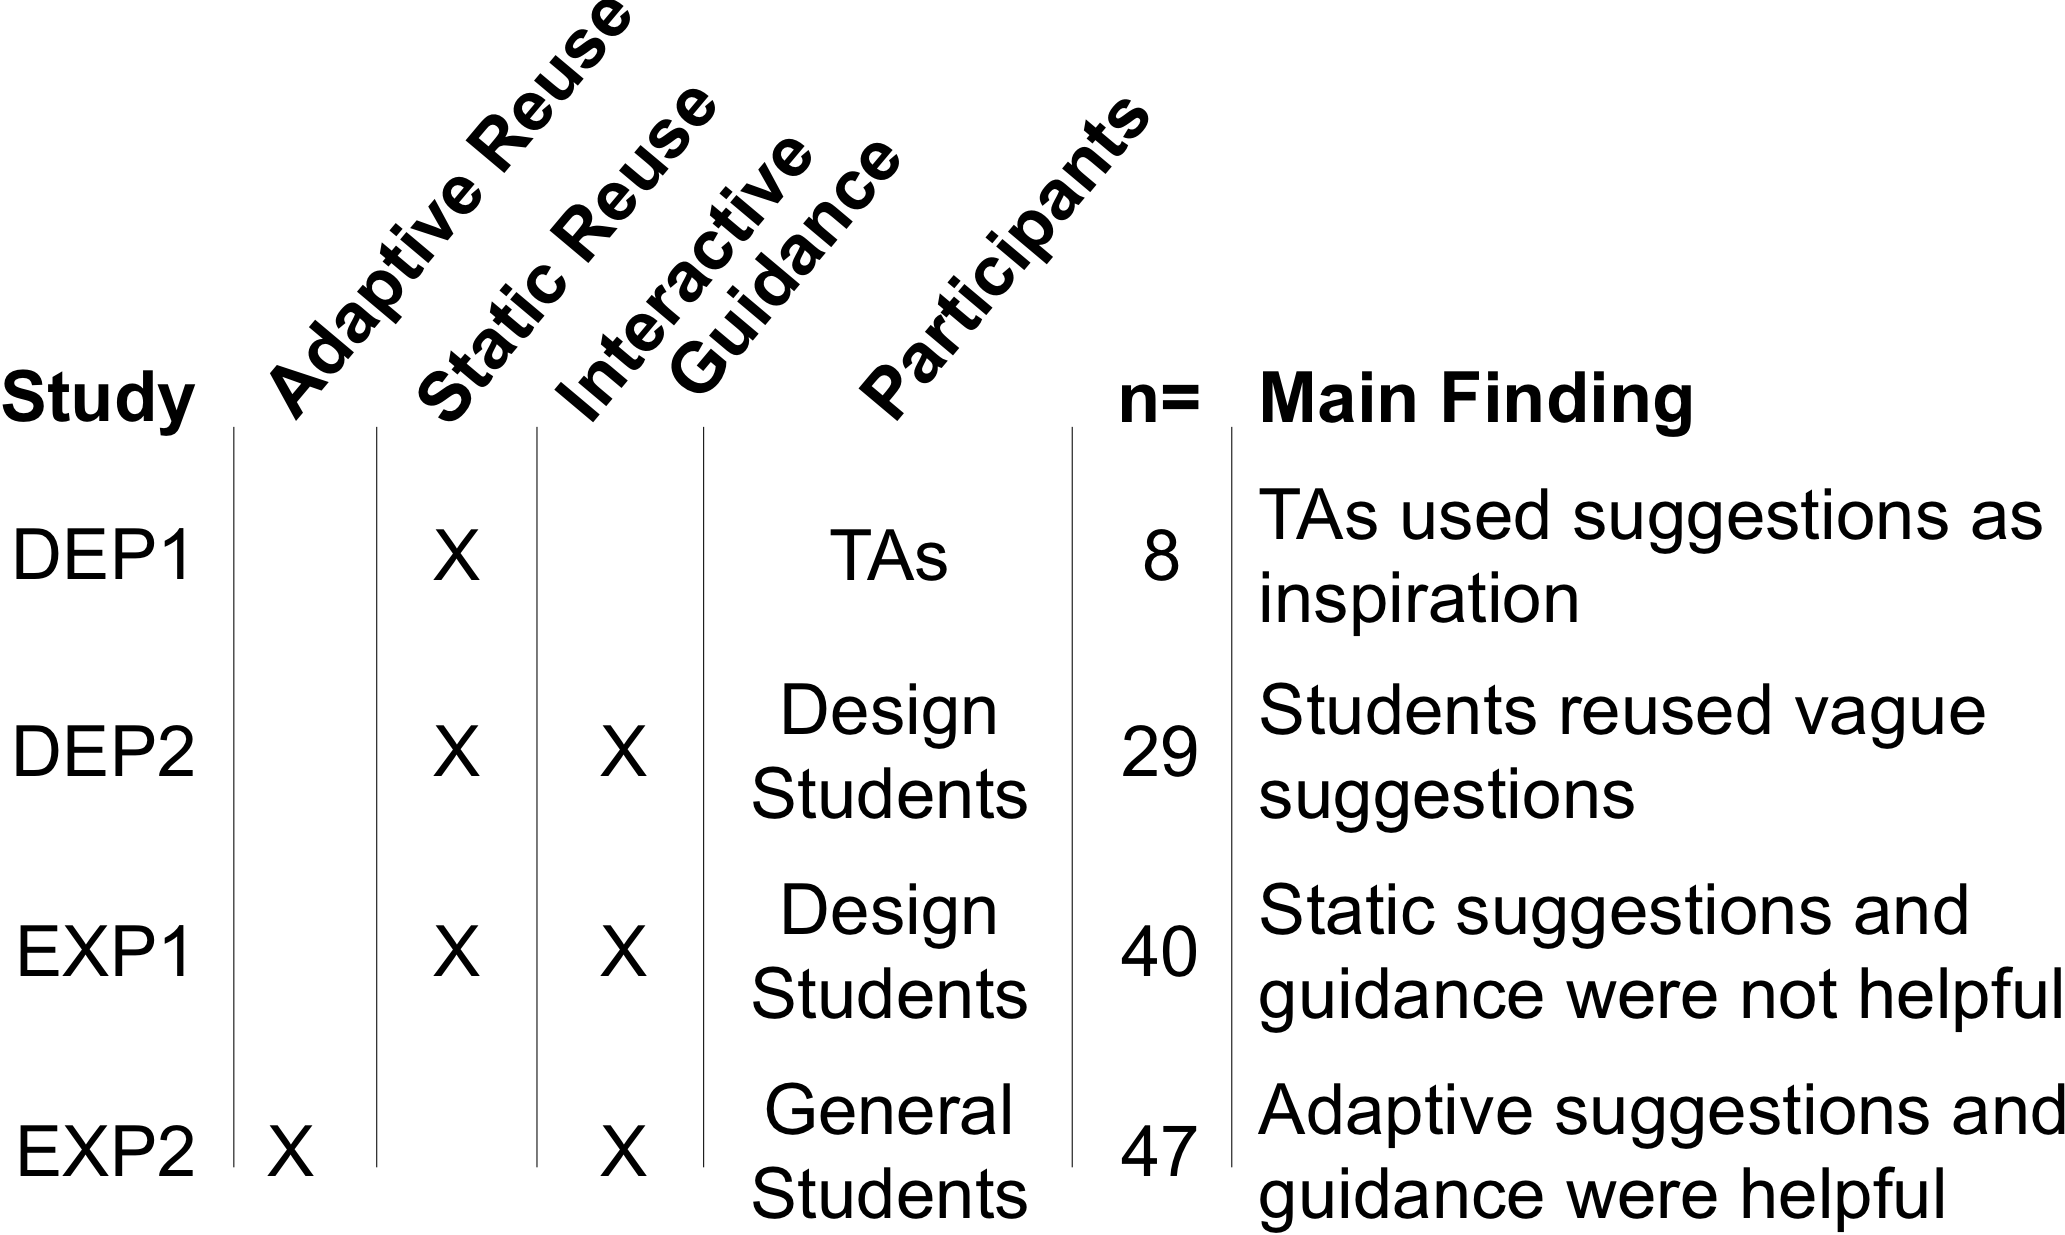
\includegraphics[width=0.6\textwidth]{critiquekit/figures/table1.png}
\end{table}


